\documentclass{article}
\usepackage[utf8x]{inputenc}
\usepackage{ucs}
\usepackage{amsmath} 
\usepackage{amsfonts}
\usepackage{upgreek}
\usepackage[english,russian]{babel}
\usepackage{graphicx}
\usepackage{float}
\usepackage{textcomp}
\usepackage{hyperref}
\usepackage{geometry}
  \geometry{left=2cm}
  \geometry{right=1.5cm}
  \geometry{top=1cm}
  \geometry{bottom=2cm}
\usepackage{tikz}
\usepackage{ccaption}
\usepackage{multicol}

\usepackage{listings}
%\setlength{\columnsep}{1.5cm}
%\setlength{\columnseprule}{0.2pt}


\begin{document}
\pagenumbering{gobble}

\lstset{
  language=C,                % choose the language of the code
  basicstyle=\linespread{1.1}\ttfamily,
  columns=fixed,
  fontadjust=true,
  basewidth=0.5em,
  keywordstyle=\color{blue}\bfseries,
  commentstyle=\color{gray},
  stringstyle=\ttfamily\color{orange!50!black},
  showstringspaces=false,
  %numbers=false,                   % where to put the line-numbers
  numbersep=5pt,
  numberstyle=\tiny\color{black},
  numberfirstline=true,
  stepnumber=1,                   % the step between two line-numbers.        
  numbersep=10pt,                  % how far the line-numbers are from the code
  backgroundcolor=\color{white},  % choose the background color. You must add \usepackage{color}
  showstringspaces=false,         % underline spaces within strings
  captionpos=b,                   % sets the caption-position to bottom
  breaklines=true,                % sets automatic line breaking
  breakatwhitespace=true,         % sets if automatic breaks should only happen at whitespace
  xleftmargin=.2in,
  extendedchars=\true,
  keepspaces = true,
}
\lstset{literate=%
   *{0}{{{\color{red!20!violet}0}}}1
    {1}{{{\color{red!20!violet}1}}}1
    {2}{{{\color{red!20!violet}2}}}1
    {3}{{{\color{red!20!violet}3}}}1
    {4}{{{\color{red!20!violet}4}}}1
    {5}{{{\color{red!20!violet}5}}}1
    {6}{{{\color{red!20!violet}6}}}1
    {7}{{{\color{red!20!violet}7}}}1
    {8}{{{\color{red!20!violet}8}}}1
    {9}{{{\color{red!20!violet}9}}}1
}


\section*{Многофайловые программы. Библиотеки}
\subsection*{Этапы сборки проекта на языке \texttt{C++}:}
\begin{enumerate}
\item \textbf{Препроцессинг}. Обрабатываются директивы компилятора \texttt{\#include}, \texttt{\#define} и другие. Удаляются комментарии. Чтобы исполнить только этот шаг, нужно передать компилятору опцию \texttt{-E}:
\begin{verbatim}
g++ -E main.cpp > preprocessed.cpp
\end{verbatim}
\item \textbf{Компиляция}: каждый файл исходного кода (файл расширения \texttt{.cpp}) транслируется в код на языке ассемблера. Чтобы исполнить только этапы препроцессинга и компиляции, нужно передать компилятору опцию \texttt{-S}:
\begin{verbatim}
g++ -S main.cpp
\end{verbatim}
\item \textbf{Ассемблирование}: каждый файл на языке ассемблера транслируется в машинный код. В результате создаётся объектный файл с расширением \texttt{.o}. Чтобы исполнить процесс до этой стадии включительно нужно передать компилятору опцию \texttt{-c}:
\begin{verbatim}
g++ -c main.cpp
\end{verbatim}
\item \textbf{Линковка}: Все объектные файлы сливаются друг с другом, а также с другими библиотеками. Даже если ваш проект состоит из одного файла, вы наверняка используйте как минимум стандартную библиотеку и на этом этапе ваш код соединяется с другими библиотеками.
\begin{verbatim}
g++ main.cpp или g++ main.o
\end{verbatim}
\end{enumerate}


\subsubsection*{Задание:}
\begin{itemize}
\item В папке \texttt{0stages} лежит исходный код простой программы. Пройдите поэтапно все стадии сборки с этой программой.
\end{itemize}

\subsection*{Сборка многофайловой программы:}
\begin{center}
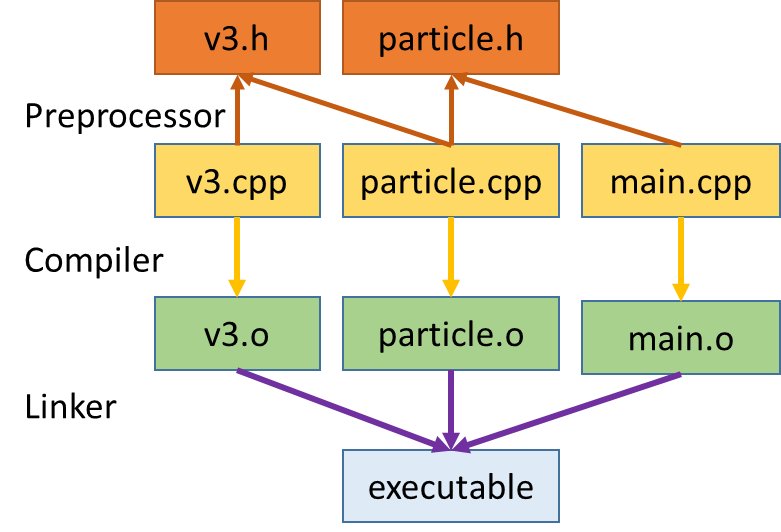
\includegraphics[scale=0.7]{../images/separate_compilation_linking.png}
\end{center}
Можно собрать всё сразу:
\begin{lstlisting}
g++ main.cpp particle.cpp v3.cpp
\end{lstlisting}
Либо можно собрать по частям:
\begin{lstlisting}
g++ -c main.cpp
g++ -c particle.cpp
g++ -c v3.cpp
g++ main.o particle.o v3.o
\end{lstlisting}

\subsection*{Виды библиотек:}
\begin{enumerate}
\item \textbf{header-only библиотеки:} Весь исходный код хранится в \texttt{.h} файле и подключается с помощью директивы \texttt{\#include} (очень просто подключить).
\item \textbf{Исходный код:} Библиотека поставляется в виде исходного кода (все \texttt{.h} и \texttt{.cpp} файлы). Для того чтобы использовать эту библиотеку, её нужно сначала скомпилировать, что может быть очень непросто для больших библиотек, так как процесс сборки может сильно отличаться на разных операционных системах и компиляторах.
\item \textbf{Статическая библиотека:} Библиотека поставляется в виде header-файлов(\texttt{.h}) и предварительно скомпилированных файлов библиотеки (\texttt{.a} или \texttt{.lib}). Эти библиотеки подключаются на этапе линковки. Такие библиотеки проще подключить к проекту, чем исходный код. Однако, вам обязательно иметь версию библиотеки, скомпилированную на той же ОС и на том же компиляторе, иначе она не подключится. Обратите внимание, что статические библиотеки обязательно должны иметь префикс \texttt{lib} и расширение \texttt{.a} (или \texttt{.lib}). Например, если мы хотим получить библиотеку под названием \texttt{image}, то файл должен называться \texttt{libimage.a}.
\item \textbf{Динамическая библиотека:} Библиотека поставляется в виде header-файлов(\texttt{.h}) и предварительно скомпилированных файлов библиотеки (\texttt{.sp} или \texttt{.dll}). Эти библиотеки подключаются на этапе \textit{выполнения программы}.
\end{enumerate}

\subsubsection*{Задания:}
\begin{itemize}
\item \textbf{header:} В папке \texttt{1image/0header-only} лежит исходный код программы, которая использует класс \texttt{Image}. Это простой класс для работы с изображениями в формате \texttt{.ppm}. Скомпилируйте и запустите эту программу.
\item \textbf{Случайные отрезки:} Используйте этот класс, чтобы создать изображение, состоящее из 100 случайных отрезков случайного цвета. Для случайных чисел используйте функцию \texttt{rand()} из библиотеки \texttt{<cstdlib>}.
\item \textbf{Случайные прямоугольники:} Добавьте в этот класс метод \\
\texttt{void draw\_rectangle(const Vector2i\& bottomleft, const Vector2i\& torright, const Color\& color)}. Используйте этот метод, чтобы создать изображение, состоящее из 100 случайных прямоуголиников случайного цвета.
\item \textbf{Шум:} Добавьте в этот класс метод \texttt{void add\_noise(float probability)}, который будет добавлять шум на картинку: каждый пиксель с вероятностью \texttt{probability} должен поменять цвет на случайный. Протестируйте этот метод на картинках.
\item \textbf{Раздельная компиляция:} В папке \texttt{1image/1separate\_compilation} лежит тот же код, но разделённый на 2 файла исходного кода. Скомпилируйте эту программу с помощью \texttt{g++}.Добавьте функции \texttt{draw\_rectangle} и \texttt{add\_noise} из предыдущих заданий в этот проект.
\item \textbf{Статическая библиотека:} Чтобы создать свою статическую библиотеку вам нужно:
\begin{enumerate}
\item Создать объектный файл необходимого исходного файла.
\item Превратить объектный файл (или файлы) в библиотеку, используя утилиту \texttt{ar}:
\begin{verbatim}
ar rvs libimage.a image.o
\end{verbatim}
\item После этого файл \texttt{libimage.a} можно будет подключить к любому другому проекту примерно так:
\begin{verbatim}
g++ main.cpp -I<путь до header-файлов> -L<путь до libimage.a> -limage
\end{verbatim}
\end{enumerate}
В папке \texttt{1image/2static\_library} лежит исходный код программы. Вам нужно создать статическую библиотеку из файла \texttt{image.cpp} и поместить полученный файл в папку \texttt{image/lib}, а header-файл поместить в папку \texttt{image/include}. Затем вам нужно удалить файл \texttt{image.cpp} и собрать программу используя только статическую библиотеку (не забывайте про опции \texttt{-I}, \texttt{-L} и \texttt{-l}).
\item \textbf{Статическая библиотека 2:} В папке \texttt{1image/3static\_test} лежит проект с одной очень маленькой статической библиотекой (содержит 1 функцию). Вам нужно собрать этот проект.
\item \textbf{Makefile:} \texttt{make} -- это специальная утилита, предназначенная для упрощения сборки проекта. В \texttt{1image/4makefile} содержится пример проекта с make-файлом. Чтобы скомпилировать его просто:
\begin{verbatim}
make <имя цели>
\end{verbatim}
либо просто
\begin{verbatim}
make
\end{verbatim}
\end{itemize}

\subsection*{Библиотека sfml:}
\end{document}